%%%%%%%%%%%%%%%%%%%%%%%%%%%%%%%%%%%%%%%%%%%%%%%%%%%%%%%%%%%%%%%%%%%%%%%%%%%%%%%%
%2345678901234567890123456789012345678901234567890123456789012345678901234567890
%        1         2         3         4         5         6         7         8
%% PP_Report.tex
%% V2.1
%% 2017/05/07
%% by Rui Santos Cruz
%% This is a skeleton file using PPIEEEtran.cls
%% (requires PPIEEEtran.cls) 
% !TEX root = ./main.tex
%%%%%%%%%%%%%%%%%%%%%%%%%%%%%%%%%%%%%%%%%%%%%%%%%%%%%%%%%%%%%%%%%%%%%%%%%%%%%%%%
\documentclass[a4paper,12pt,journal,twoside,compsoc]{PPIEEEtran}

% In the ReportType command chose "act" for Activity Report or "learn" for Learnings Report
\newcommand*{\ReportType}{act}
% -----------------------------------------------------------------------------
% The Preamble document contains all the necessary Packages for typesetting
% Modify it to suit your needs
% -----------------------------------------------------------------------------
%%%%%%%%%%%%%%%%%%%%%%%%%%%%%%%%%%%%%%%%%%%%%%%%%%%%%%%%%%%%%%%%%%%%%%%%%%%%%%%%
%2345678901234567890123456789012345678901234567890123456789012345678901234567890
%        1         2         3         4         5         6         7         8
% Required Packages and commands
% --> Please Choose the MAIN LANGUAGE for the document in package BABEL (below)
% --> Please Choose the TYPE OF REPORT for the document in \ReportType (below)
% !TEX root = ./main.tex
% PP_Report_Preamble.tex
% V2.1
% 2017/05/07
% by Rui Santos Cruz
%%%%%%%%%%%%%%%%%%%%%%%%%%%%%%%%%%%%%%%%%%%%%%%%%%%%%%%%%%%%%%%%%%%%%%%%%%%%%%%%
%
% *** INPUT LANGUAGE PACKAGES ***
% Choose the main language in package Babel
\usepackage[english,main=portuguese]{babel}
\usepackage[utf8]{inputenc}
\usepackage{iflang}

% *** ACRONYM PACKAGES ***
% Put definition of Acronyms at the end of the document
\usepackage[printonlyused,nolist]{acronym}

% *** CITATION PACKAGES ***
\usepackage{cite}

% *** GRAPHICS RELATED PACKAGES ***
\usepackage[pdftex]{graphicx}
\DeclareGraphicsExtensions{.pdf,.jpeg,.png}

% *** MATH PACKAGES ***
\usepackage[cmex10]{amsmath}

% *** SPECIALIZED LIST PACKAGES ***
\usepackage{algorithmic}

% *** ALIGNMENT PACKAGES ***
\usepackage{array}

% *** SUBFIGURE PACKAGES ***
\usepackage[caption=false,font=normalsize,labelfont=sf,textfont=sf]{subfig}

% *** FLOAT PACKAGES ***
\usepackage{fixltx2e}

% *** PDF, URL AND HYPERLINK PACKAGES ***
\usepackage{url}

% *** BACKGROUND Material ***
\usepackage{eso-pic}
\usepackage[
  contents={},
  opacity=1,
  scale=1,
  color=blue!90
  ]{background}
  
% *** CONDITIONALS ***
\usepackage{ifthen}

% Clever Referencing
% Note: portuguese is supported through "brazilian" option
\usepackage[\IfLanguageName{english}{english}{brazilian}]{cleveref}

%%%%%%%%%%%%%%%%%%%%%%%%%%%%%%%%%%%%%%%%%%%%%%%%%%%%%%%%%%%%%%%%%%%%%%%%%%%%%%%%
% PLEASE DO NOT CHANGE THIS SECTION
% Printing the Scoring Table
\AddToShipoutPicture*{\BackgroundPic}
%%%%%%%%%%%%%%%%%%%%%%%%%%%%%%%%%%%%%%%%%%%%%%%%%%%%%%%%%%%%%%%%%%%%%%%%%%%%%%%%
% PLEASE DO NOT CHANGE THIS SECTION
% Print Vertical Identifications on even and odd pages
\AddEverypageHook{%
  \ifthenelse{\isodd{\value{page}}}%
  {\backgroundsetup{
    angle=90,
    position={-0.1\textwidth,-1.055\textheight},
    contents={\tiny{PP-2017 V2.1}}
    }% Odd Pages
  }%
  {\backgroundsetup{
    angle=90,
    position={0.97\textwidth,-1.05\textheight},%
    contents={\ifthenelse{\equal{\ReportType}{act}}{%
              \tiny{\tlangRepActivity}}{\tiny{\tlangRepLearning}}}
    }% Even Pages
  }%
  \BgMaterial}
  %%%%%%%%%%%%%%%%%%%%%%%%%%%%%%%%%%%%%%%%%%%%%%%%%%%%%%%%%%%%%%%%%%%%%%%%%%%%%%%%
% correct bad hyphenation here
\hyphenation{op-tical net-works semi-conduc-tor}
%%%%%%%%%%%%%%%%%%%%%%%%%%%%%%%%%%%%%%%%%%%%%%%%%%%%%%%%%%%%%%%%%%%%%%%%%%%%%%%%
%2345678901234567890123456789012345678901234567890123456789012345678901234567890
%        1         2         3         4         5         6         7         8
\begin{document}

%%%%%%%%%%%%%%%%%%%%%%%%%%%%%%%%%%%%%%%%%%%%%%%%%%%%%%%%%%%%%%%%%%%%%%%%%%%%%%%%
%2345678901234567890123456789012345678901234567890123456789012345678901234567890
%        1         2         3         4         5         6         7         8
%% PP_Report_Cover.tex
%% V2.1
%% 2017/05/07
%% by Rui Santos Cruz
% !TEX root = ./main.tex
%%%%%%%%%%%%%%%%%%%%%%%%%%%%%%%%%%%%%%%%%%%%%%%%%%%%%%%%%%%%%%%%%%%%%%%%%%%%%%%%
% paper title
% can use linebreaks \\ within to get better formatting as desired
% Do not put math or special symbols in the title.
\title{Deteção de eventos em discursos políticos}

%%%%%%%%%%%%%%%%%%%%%%%%%%%%%%%%%%%%%%%%%%%%%%%%%%%%%%%%%%%%%%%%%%%%%%%%%%%%%%%%
% Author names
%
% note positions of commas and nonbreaking spaces ( ~ ) LaTeX will not break
% a structure at a ~ so this keeps an author's name from being broken across
% two lines.
% use \thanks{} to gain access to the first footnote area
% a separate \thanks must be used for each paragraph.
%
%\IEEEcompsocitemizethanks is a special \thanks that produces the bulleted
% lists for "first footnote" author affiliations. 
% Use \IEEEcompsocthanksitem which works much like \item
% for each affiliation group.
\author{Gonçalo~Fialho~Pires,
        Pedro~Miguel~Duarte% <-this % stops a space
% Change the Course Name 
% note: need leading \protect in front of \\ to get a newline within \thanks as
% \\ is fragile and will error, could use \hfil\break instead.
\IEEEcompsocitemizethanks{
\IEEEcompsocthanksitem Gonçalo~Fialho~Pires, nr. 79112,\protect\\ 
E-mail: goncalo.f.pires@tecnico.ulisboa.pt,
\IEEEcompsocthanksitem Pedro~Duarte, nr. 78328,\protect\\
E-mail: pedro.m.duarte@tecnico.ulisboa.pt,\protect\\
Instituto Superior Técnico, Universidade de Lisboa.\protect\\}% <-this % stops an unwanted space}% <-this % stops an unwanted space
\thanks{Manuscrito recebido a 1 de Junho de 2018.}
}
%%%%%%%%%%%%%%%%%%%%%%%%%%%%%%%%%%%%%%%%%%%%%%%%%%%%%%%%%%%%%%%%%%%%%%%%%%%%%%%%
% The paper headers
\markboth{Deteção de eventos em discursos políticos}%
% for a single student
%{Surname}% : for a single student 
% for a Group Report 
{Duarte \MakeLowercase{\textit{et al.}}}% : for a Group Report 
%
% The only time the second header will appear is for the odd numbered pages
% after the title page when using the twoside option.

%%%%%%%%%%%%%%%%%%%%%%%%%%%%%%%%%%%%%%%%%%%%%%%%%%%%%%%%%%%%%%%%%%%%%%%%%%%%%%%%
% Prints in Subtitle the type of Report
% PLEASE DO NOT CHANGE THIS SECTION
\IEEEspecialpapernotice{%
\ifthenelse{\equal{\ReportType}{act}}{%
\tlangRepActivity}{\tlangRepLearning}
}
%%%%%%%%%%%%%%%%%%%%%%%%%%%%%%%%%%%%%%%%%%%%%%%%%%%%%%%%%%%%%%%%%%%%%%%%%%%%%%%%
%%%%%%%%%%%%%%%%%%%%%%%%%%%%%%%%%%%%%%%%%%%%%%%%%%%%%%%%%%%%%%%%%%%%%%%%%%%%%%%%
% The paper Abstract and Keywords
\IEEEtitleabstractindextext{%

\begin{abstract}

This report will discuss the objectives of the Global Game Jame edition of 2018 and its correspondent Independent Studies 1 activity, as well as describe the tasks I have been assigned to and how I executed them. Furthermore, it will also report the results objectively of each of the assigned tasks. 

\end{abstract}
%
\begin{IEEEkeywords}
Soft-skills, Event Organization
\end{IEEEkeywords}}
%%%%%%%%%%%%%%%%%%%%%%%%%%%%%%%%%%%%%%%%%%%%%%%%%%%%%%%%%%%%%%%%%%%%%%%%%%%%%%%%

% make the title area
\maketitle

\IEEEdisplaynontitleabstractindextext
\IEEEpeerreviewmaketitle
%%%%%%%%%%%%%%%%%%%%%%%%%%%%%%%%%%%%%%%%%%%%%%%%%%%%%%%%%%%%%%%%%%%%%%%%%%%%%%%%
%%%%%%%%%%%%%%%%%%%%%%%%%%%%%%%%%%%%%%%%%%%%%%%%%%%%%%%%%%%%%%%%%%%%%%%%%%%%%%%%
\section{Introduction}
% The very first letter is a 2 line initial drop letter followed
% by the rest of the first word in caps (small caps for compsoc).
% 
% form to use if the first word consists of a single letter:
% \IEEEPARstart{A}{demo} file is ....
% 
% Here we have the typical use of a "E" for an initial drop letter
% and "STE" in caps to complete the first word.


\IEEEPARstart{T}{he} \ac{GGJ} is a non-profit worldwide event, i.e. it happens all around the world, in multiple physical locations, at the same time, and strives to grow the idea of creation and team spirit. It allows for people to come together with a common goal in mind: creating a game within a period of 48 hours. In Lisbon, one of these physical locations of the event is at the Taguspark campus of \ac{IST}, which is collaborating with the Faculdade de Belas Artes da Universidade de Lisboa.

While this event goal is to focus on people's creativity, encourage teamwork and inspire developers, it is also a great opportunity to meet new people, make new friends and establish contact with game companies, for example Miniclip that sponsored the event (in the Taguspark) of last year edition.

Because the actual event is only on the weekend of 26-28 of January, in 2018, that part of the activity (which I am still going to be taking part of) will not be described. However, because I participated in the previous edition as a Jammer (as a participant, making a game) and one of my colleagues was part of the organization in the logistics team, I have an idea of what I am going to be doing on the actual event and of what to expect. As such, I will also describe briefly what it is that I am expecting from the actual event.

In the rest of this report, I will describe the objectives of this activity as well as the planning and preparation behind it. I will also describe the tasks that I did in this activity. Finally, I will provide a critic overview of the results as well the upcoming actual event.

The organization of this document is as follows: \cref{objectives} describes the objectives behind this activity; \cref{tasks} discusses the tasks that I did on the scope of the activity; \cref{results} provides an objective report of the results that resulted from the tasks described in the previous sections. Finally, \cref{concl} concludes this report.

%%%%%%%%%%%%%%%%%%%%%%%%%%%%%%%%%%%%%%%%%%%%%%%%%%%%%%%%%%%%%%%%%%%%%%%%%%%%%%%%
\section{Objectives}
\label{objectives}

The objective of this activity was to help in the organization of the Global Game Jam 2018, in the Taguspark campus. More specifically, the task I was assigned to originally to the logistics team, i.e. I was to support the participants and the rest of the organization on the days of the event, in January 26-28. 

Helping the participants means showing them where the rooms are, where they will sleep, where they will work, as well as helping them choose their own teams if they attend the event without one - this is a common occurrence; because it is in the spirit of the GGJ to bond with other people, some people come without any teams formed and do so on the day of the event.

Helping the organization means to help them prepare for the day of the event. This was done in the form of "filling in the gaps", i.e. anything the organization were short on, I would help them on that. Because of this, instead of just being a part of the logistics team, I was also assigned to the sponsors team and the inventory team.

The purpose of the Global Game Jam, as a whole, is to incentive people to be creative. Due to the nature of the event having a very limited time to make a game with a specific theme as complete and playable as possible, it forces the participants to not worry to much on the details and just let the creativity and ideas flow in order to shape something that can be considered both a game and a piece of art in 48 hours. It focuses a lot on the teamwork aspect as well, by encouraging participants without a team to find their partners in a session previous to the game, i.e. a participant that is a programmer from IST might want to talk to participants from the \ac{FBAUL} to find designers or sound designers, which will complement the skills of each other. Thus, it promotes the meeting of new people.

Furthermore, because after the event there will be a showcasing of the games that were made by the teams, companies can also use this event to spot new talents in the game industry, and teams that were made specifically for participating in this event might find themselves wanting to stay together to participate in further Global Game Jams or even make their own game outside of this event.

Also note that the theme of the game is only known globally some hours before the Jam begins. This ensures that participants do not make a game beforehand and go into the event with a complete game already made. Furthermore, it forces the participants to be quick on their thinking and discuss ideas with their team members, and even other teams, on the fly. 

%%%%%%%%%%%%%%%%%%%%%%%%%%%%%%%%%%%%%%%%%%%%%%%%%%%%%%%%%%%%%%%%%%%%%%%%%%%%%%%%
%%%%%%%%%%%%%%%%%%%%%%%%%%%%%%%%%%%%%%%%%%%%%%%%%%%%%%%%%%%%%%%%%%%%%%%%%%%%%%%%
\section{Tasks}
\label{tasks}

In this section I will describe the tasks I was assigned in this activity, as well as explain how I executed them. The tasks will be divided by team, as I am part of three of the teams of the organization and each of them has a specific work flow and purpose.

\subsection{Sponsors Team}

The purpose of the sponsors team is to find potential companies that would be interested in sponsoring the event in the IST and contacting them. 

We did this by first looking at the necessary items that we would need a large quantity of, for example: food, coffee, water and other beverages, etc. One of the members thought it would be interesting to find a sponsor of Lazy Bags, an item that inflates with air just by opening it and having it move. This idea came from the fact that since the event has a period of 48 hours, participants would need to sleep or rest somewhere. Although many participants go home to rest if their house is close by, or sleep at their friends house, a lot just rests in the assigned room for this purpose in the Taguspark, but they would still need some kind of sleeping bag. Thus, I searched online for LazyBags, found a Portuguese company that seemed to have a lot of these and contacted them via email to ask if they would sponsor us.

We also established contact with other companies like Pingo Doce for some food and beverages, and Maggi for noodles.

\subsection{Inventory Team}

The objective of the inventory team (or shopping team) is to keep track of the things that will be needed during the event and plan ahead to buy them. We are required to make an estimate of the quantity of each items will be needed and elaborate a budget. 

The items included food and beverages, as previously explained, but also posters, banners, cards, mugs and t-shirts or sweatshirts. This means we had to find services that print specific types of promotional posters and banners, as wells as business-like cards that are wore around the neck. Mugs and t-shirts are for promoting the IST Game Lab ("Laboratório de Jogos do IST") during the event, and the banners and posters for promoting the Global Game Jam event to get as many people as possible participating; the banners and posters will be put up in the IST and FBAUL faculties. The cards are for the identification of the staff during the actual event and will be necessary so participants know to whom to turn when in need of any kind of assistance.

One of the great challenges of the task of shopping and budgeting is finding the right products and items at affordable prices and, from my experience with this activity, it is better to not do this kind of task alone. This is due to the fact that one person alone will easily skip some places that could have better or cheaper items. Furthermore, when people are looking for things to buy that have already been discussed and declared as important for the event, one can occasionally find a new type of item that would be interesting to have in an event like this. Such is the case of a trophy: usually, after the 48 hours of game development are over, there is a showcasing (after a short break) where participants show their game to the rest of the Jammers, and after the showcase, people vote on the game they liked the most. In the previous edition, the most voted game gained a symbolic prize (a 80 euros steam card to spend on the Steam platform - to buy games, etc.). While browsing for items, one of the members of the team thought it would be interesting to also give away a trophy as a keepsake. Note that this event is not supposed to be competitive and we encourage cooperation even between teams; because of this, we only announce that there is a prize after the games are made.

\subsection{Logistics Team}

The task that is assigned to the logistics team is only done in the days of the event and also a bit prior to that. As such, I cannot report what I did on this matter. I know, however, what will be expected of me and some of the problems that may arise, because I already participated in the previous edition as a Jammer but I watched closely what the team did. 

As a member of the logistics team, I will need to move objects in and out of the rooms in order to prepare them for the participants to be as comfortable as possible and be able to focus entirely on participating. This means tidying up rooms, moving tables and chairs and moving electrical plugs so that the participants can plug in their computers.

Furthermore, I may also need to be alert to any incident that may happen so the security team of the IST faculty can rapidly and efficiently intervene. I also must answer questions any participant may have during the event.


%%%%%%%%%%%%%%%%%%%%%%%%%%%%%%%%%%%%%%%%%%%%%%%%%%%%%%%%%%%%%%%%%%%%%%%%%%%%%%%%
%%%%%%%%%%%%%%%%%%%%%%%%%%%%%%%%%%%%%%%%%%%%%%%%%%%%%%%%%%%%%%%%%%%%%%%%%%%%%%%%


\section{Results}
\label{results}

Analogously to \cref{tasks}, this section will be divided in three parts, one for each of the teams I am a part of. For each team, the results will be reported in its corresponding section.

\subsection{Sponsors Team}

Up to this date, no sponsor that I have established contact responded to my request. However, we already have others entities that agreed to sponsor us.
Objectively, I believe some potential sponsors did not yet respond to our request because the period of time that passed between the request and the date of submission of this report was not too long.

\subsection{Inventory Team}

A large part of the budget is, to this date, mostly done. This means the printing jobs, such as the banners and the posters, are budgeted and ready to be ordered, and so are the t-shirts which will also have to be stamped.

Overall, we found some important products with cheap prices that will be bought soon after this report's due date.

\subsection{Logistics Team}

There are no results to report in the scope of the logistics team as any tasks in relevant to this team will only be done after the due date of this report.


\section{\IfLanguageName{english}{Conclusion}{Conclusão}}
\label{concl}
Overall, I am very pleased on how things turned out, since a good amount of work is already done before the event even starts, and this shows just how much preparation is needed and how much teamwork and communication is necessary to make things go smoothly. 

Also please note that because the event did not yet occur on the date I am writing this - and because it will only occur in January of 2018 - there is not much to report about the part of the activity that I will do then. However, it is to note that many hours of work have already been put into this activity by preparing the inventory and establishing contact with potential sponsors, as well as communicating with the rest of the organization team and helping wherever needed.

%%%%%%%%%%%%%%%%%%%%%%%%%%%%%%%%%%%%%%%%%%%%%%%%%%%%%%%%%%%%%%%%%%%%%%%%%%%%%%%%
%%%%%%%%%%%%%%%%%%%%%%%%%%%%%%%%%%%%%%%%%%%%%%%%%%%%%%%%%%%%%%%%%%%%%%%%%%%%%%%%
% use section* for acknowledgement
\ifCLASSOPTIONcompsoc
  % The Computer Society usually uses the plural form
  \section*{\IfLanguageName{english}{Acknowledgments}{Agradecimentos}} % Acknowledgments
\else
  % regular IEEE prefers the singular form
  \section*{Acknowledgment}
\fi

I would like to thank professor Carlos Martinho for allowing me to become a part of the organization of the \ac{GGJ} of the Taguspark, and my fellow colleagues for working with me.
%%%%%%%%%%%%%%%%%%%%%%%%%%%%%%%%%%%%%%%%%%%%%%%%%%%%%%%%%%%%%%%%%%%%%%%%%%%%%%%%

%%%%%%%%%%%%%%%%%%%%%%%%%%%%%%%%%%%%%%%%%%%%%%%%%%%%%%%%%%%%%%%%%%%%%%%%%%%%%%%%
% biography section
% 

\begin{IEEEbiography}[{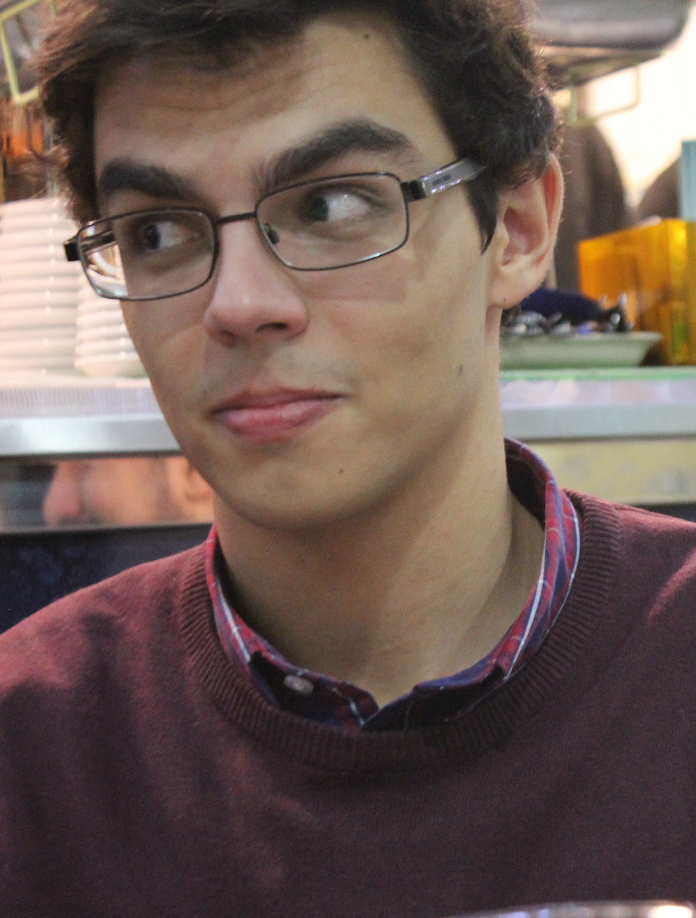
\includegraphics[width=1in,height=1.25in,clip,keepaspectratio]{me.png}}]{Pedro Miguel dos Santos Duarte}
I am currently pursuing my Master's Degree in Engineering studies at \ac{IST}, specializing in Intelligent Systems and Information Systems. I strive to make this world a better place for everybody living in it and I am always ready to take on a challenge.
\end{IEEEbiography}

%%%%%%%%%%%%%%%%%%%%%%%%%%%%%%%%%%%%%%%%%%%%%%%%%%%%%%%%%%%%%%%%%%%%%%%%%%%%%%%%

% *** DEFINITION OF ACRONYMS ***
	\acrodef{GGJ}{Global Game Jam}
	\acrodef{IST}{Instituto Superior Técnico}
    \acrodef{FBAUL}{Faculdade de Belas Artes da Universidade de Lisboa }
	
% that's all folks
\end{document}